\documentclass{article}

% if you need to pass options to natbib, use, e.g.:
%     \PassOptionsToPackage{numbers, compress}{natbib}
% before loading neurips_2021

% ready for submission

\PassOptionsToPackage{numbers, square, sort&compress}{natbib}
\usepackage{neurips_2021}

% to compile a preprint version, e.g., for submission to arXiv, add add the
% [preprint] option:
%     \usepackage[preprint]{neurips_2021}
% https://www.overleaf.com/project/5f05abd2e41db100011026fc
% to compile a camera-ready version, add the [final] option, e.g.:https://www.overleaf.com/project/5f05abd2e41db100011026fc
%     \usepackage[final]{neurips_2021}

% to avoid loading the natbib package, add option nonatbib:
%    \usepackage[nonatbib]{neurips_2021}

\usepackage[utf8]{inputenc} % allow utf-8 input
\usepackage[T1]{fontenc}    % use 8-bit T1 fonts
\usepackage{hyperref}       % hyperlinks
\usepackage{url}            % simple URL typesetting
\usepackage{booktabs}       % professional-quality tables
\usepackage{amsfonts}       % blackboard math symbols
\usepackage{nicefrac}       % compact symbols for 1/2, etc.
\usepackage{microtype}      % microtypography
\usepackage{xcolor}         % colors


\usepackage{amssymb, bm, blkarray, multicol}
\usepackage{listings,lmodern}
\usepackage{graphicx}
\usepackage{enumitem}
\usepackage{algorithm}
\usepackage{algpseudocode}
\usepackage[nottoc]{tocbibind}
\usepackage{upgreek}

\usepackage{tikz}

\usepackage{mathtools}
\mathtoolsset{showonlyrefs}

\usepackage{latexsym}

\usepackage{physics} 

\newtheorem{theorem}{THEOREM}
\newtheorem{lemma}[theorem]{LEMMA}
\newtheorem{corollary}[theorem]{COROLLARY}
\newtheorem{proposition}[theorem]{PROPOSITION}
\newtheorem{remark}[theorem]{REMARK}
\newtheorem{definition}[theorem]{DEFINITION}
\newtheorem{fact}[theorem]{FACT}

\newtheorem{problem}[theorem]{PROBLEM}
\newtheorem{exercise}[theorem]{EXERCISE}
\def \set#1{\{#1\} }

\newcommand{\E}{\mathbb{E}}
\renewcommand{\var}{\mathrm{Var}}
\newcommand{\cov}{\mathrm{Cov}}
\newcommand{\KL}{\mathrm{KL}}
\newcommand{\neighb}{\text{ne}}
% \DeclareMathOperator*{\argmax}{arg\,max}
% \DeclareMathOperator*{\argmin}{arg\,min}
\newcommand{\Perp}{\mathrel{\text{\scalebox{1.07}{$\perp\mkern-10mu\perp$}}}}
\newcommand{\tildepi}{\tilde{\pi}}
\newcommand{\argdot}{{\,\vcenter{\hbox{\tiny$\bullet$}}\,}}%
% for comments
\newcommand{\hksay}[1]{[\textcolor{green!70!black}{\textbf{HK: }}\textcolor{green!50!black}{#1}]}
\newcommand{\ajsay}[1]{[\textcolor{red!70!black}{\textbf{AJ: }}\textcolor{red!50!black}{#1}]}

\renewcommand{\bibname}{References}
\global\long\def\given{\vert}%
\bibliographystyle{apalike}

\title{
    Nonparametric diagnostics for MCMC implementations: revisiting Geweke's test
}

% The \author macro works with any number of authors. There are two commands
% used to separate the names and addresses of multiple authors: \And and \AND.
%
% Using \And between authors leaves it to LaTeX to determine where to break the
% lines. Using \AND forces a line break at that point. So, if LaTeX puts 3 of 4
% authors names on the first line, and the last on the second line, try using
% \AND instead of \And before the third author name.

\author{%
  David S.~Hippocampus\thanks{Use footnote for providing further information
    about author (webpage, alternative address)---\emph{not} for acknowledging
    funding agencies.} \\
  Department of Computer Science\\
  Cranberry-Lemon University\\
  Pittsburgh, PA 15213 \\
  \texttt{hippo@cs.cranberry-lemon.edu} \\
  % examples of more authors
  % \And
  % Coauthor \\
  % Affiliation \\
  % Address \\
  % \texttt{email} \\
  % \AND
  % Coauthor \\
  % Affiliation \\
  % Address \\
  % \texttt{email} \\
  % \And
  % Coauthor \\
  % Affiliation \\
  % Address \\
  % \texttt{email} \\
  % \And
  % Coauthor \\
  % Affiliation \\
  % Address \\
  % \texttt{email} \\
}

\begin{document}

\maketitle

\iffalse
\begin{abstract}
    The Geweke diagnostic is a popular technique that assesses whether a Markov chain
  algorithm samples a posterior correctly: it
  generates samples from a joint distribution in two ways,
  one that involves the sampler and one that does not, and compares
  the two using a hypothesis test. 
  It can in principle detect any type of error---lack of
  convergence, but also implementation errors, derivation errors, or
  insufficient lag. A practical limitation is the requisite
  two-sample test: For multivariate distributions on Euclidean space, the method typically compares a list of test statistics, such as first and second moments.
  It can be difficult to apply in machine learning, where spaces are not necessarily  
  Euclidean (e.g., graphs, text) and the distinction
  between parameters and latent variables blurs. 
  To broaden the method's scope, we cast the test as a sample  estimate of a probability metric, which we implement as maximum mean discrepancy (MMD). 
  The resulting test is nonparametric,
  benefits from the kernel trick to compute the metric without
  optimization, can be applied on any domain by plugging in a suitable
  kernel, and lets users draw on a large arsenal of established
  results to select a kernel. 
  In experiments, we showcase its performance on a variety of problems involving plausible implementation mistakes.
%   We demonstrate its performance on non-Euclidean domains,
%   such as graphs, and show that it performs competitively even in the Euclidean case, albeit at
%   higher computational cost than some available alternatives.
\end{abstract}
\fi
% \begin{abstract}
%     The Geweke diagnostic is a popular technique that assesses whether a Markov chain
%   algorithm samples a posterior correctly: it
%   generates samples from a joint distribution in two ways,
%   one that involves the sampler and one that does not, and compares
%   the two using a two-sample hypothesis test. 
%   The test detects a wide variety of errors:
%   lack of
%   convergence, implementation errors, derivation errors, or
%   insufficient lag.
%   Implementations of  the two-sample test have generally required
%   user-designed test statistics, making them challenging to generalize to modern ML settings with complex, structured variables,
%   such as strings and graphs.
%   We cast the test statistic as a sample  estimate of a probability metric, which we implement as a maximum mean discrepancy (MMD).
% The resulting nonparametric test statistic is defined via a reproducing kernel, and we can draw on a  large arsenal of established  results for kernel choice.
%   In experiments, we showcase test performance on a variety of problems involving plausible implementation mistakes.
% \end{abstract}  

\begin{abstract}
The Geweke diagnostic is a popular technique that assesses whether a Markov chain
  algorithm samples a posterior correctly: it
  generates samples from a joint distribution in two ways,
  one that involves the sampler and one that does not, and compares
  the two using a two-sample hypothesis test. 
  The test detects a variety of errors: lack of
  convergence, but also mistakes in implementation or derivation.
  However, it requires the user to hand-craft a set of test statistics, which makes it 
  challenging to apply to all but the simplest models.
%   However, it relies on
%   user-designed test statistics, making it challenging to generalize to modern machine learning settings with complex, structured variables
%   such as strings and graphs.
  We cast the test statistic as a sample estimate of a probability metric, which we implement as a maximum mean discrepancy (MMD).
The resulting test is nonparametric, its test statistic can be evaluated via a reproducing kernel, and the user can draw on a large arsenal of established results to choose an appropriate kernel for the setting.
  In experiments, we showcase test performance on a variety of problems involving plausible implementation mistakes.
\end{abstract}  


\section{Introduction}
\label{section:intro}

Consider an unobserved
random variable $\Theta$ (a Bayesian model parameter, or a latent variable)
an observed random variable $Y$, and a task involving the
posterior distribution of $\Theta$ given $Y$. If the posterior cannot
be calculated analytically, Markov chain Monte Carlo sampling
(MCMC) is often the method of choice.
The Geweke diagnostic attempts to determine
whether the algorithm generates samples from the correct distribution
\cite{geweke_getting_2004}.
The goal is to detect errors from any source, including 
implementation mistakes, wrong assumptions in the
derivation, or sequential dependence induced by collecting samples from the chain too
frequently.
That is not quite the same as a convergence diagnostic \citep[see e.g.][]{robert_short_2011}, which tests whether
sampler has converged to its stationary distribution, but assumes the sampler itself
is correct.

Geweke's approach is simple and ingenious:
Assume a model with 
likelihood $p(y|\theta)$, prior density $\pi(\theta)$, and posterior
$\pi(\theta|y)$. The MCMC algorithm generates samples from an
approximate posterior $\tilde{\pi}(\theta|y)$. Our goal is to 
determine whether $\tilde{\pi}(\theta|y)=\pi(\theta|y)$. 
Since $p(y|\theta)$ and $\pi(\theta)$ are known, one can generate
samples from the exact joint distribution of $(Y,\Theta)$ as
\begin{equation}
  \Theta_i\sim \pi
  \quad\text{ and }\quad
  Y_i\sim p(\argdot|\Theta_i)\quad\text{ for }i=1,\ldots,n\;.
  \label{eq:ancestralsampling}
\end{equation}
Call this the \emph{forward factorization} of the joint distribution.
Alternatively, one can use the \emph{backward factorization}
\begin{equation*}
  Y'_i\sim p(\argdot)=\int p(\argdot|\theta)\pi(\theta)d\theta
  \quad\text{ and }\quad
  \Theta'_i\sim\tilde{\pi}(\argdot|Y'_i)\;.
\end{equation*}
(Note $Y'_i$ can be generated by drawing a pair, say $(Y_i',\Theta_i'')$, from the forward joint,
and discarding $\Theta_i''$.) The sampler is correct if, and only if, $\{(Y_1,\Theta_1),\ldots,(Y_n,\Theta_n)\}$
and $\{(Y_1',\Theta_1'),\ldots,(Y_n',\Theta_n')\}$ have the same distribution; 
% Whether that is the case is determined using a
the query is answered using a hypothesis test.

There is no free lunch: The approximate posterior
$\tilde{\pi}(\argdot|Y_i)$ in the backward factorization
is represented by the sampler, which must burn in for \emph{each}
value of $Y_i$. Such separate burn-ins are costly; starting with a previous value to reduce time spent in burn-in (as proposed by \cite{geweke_getting_2004}) is possible, 
but turns the diagnostic as a whole into a Markov chain,
 which in turn must converge, as pointed by \citet{talts_validating_2018}.
% See Section \ref{related:work} for references on the problem, and on mitigation strategies.
Nonetheless, Geweke's method has proven useful in practice, and can pick up
on suprisingly subtle mistakes.
It has been invoked, for example, by \citet{del_negro_time_2015} and
\citet{karlsson_corrigendum_2017} to correct two highly cited MCMC
algorithms in the econometrics literature, over a decade after their
initial publications.
As noted by \citet{grosse_testing_2014}, one may easily check that each of the sampler's steps preserves detailed balance, but a few errors may still slip through. 
In our own experience, it is often the detection of coding-,
derivation-, and other ``human'' errors where the Geweke diagnostic really
shines, and we would argue that it should be used as a complement to
mixing diagnostics, not as a replacement.

% \textcolor{red}{remainder of section 1: One (short) paragraph
%   summarizing what we do}
In the following, we generalize Geweke's approach by framing it in terms of distance between joint distributions. We discuss a suitable distance, Maximum Mean Discrepancy (MMD), that makes it applicable with minimal user effort whenever a kernel is available for the given problem domain. We combine MMD with two joint sampling methods, yielding two MCMC diagnostic tests, and demonstrate their efficacy relative to the Geweke test and more recent benchmarks in several experiments.

% % Markov chain Monte Carlo (MCMC) is an indispensable tool in modern Bayesian analysis, where a great majority of models have intractable posteriors and require simulation.
% Suppose we are faced with a Bayesian inference problem. 
% We model observed data $\bar{y}$ with a model $p(y|\theta)$, which is parameterized by $\theta\in \Theta$. 
% Given our observations, we wish to update our prior belief $\pi(\theta)$ and compute the posterior $\pi(\theta|y)=p(y|\theta)\pi(\theta)/p(y)$. 
% \footnote{For simplicity, we consider only probability distributions specified by densities with respect to the Lebesgue measure, and the extension to general measures is a routine.} 
% Apart from simple models, calculating the normalizer $p(y)=\int p(y\given \theta) \pi(\theta) \dd \theta$ is intractable, and the posterior is not given in closed form.
% Instead, we simulate the posterior by drawing samples from a Markov Chain with $\pi(\theta|y)$ as its stationary distribution using a Markov Chain Monte Carlo (MCMC) algorithm  \citep{metropolis_equation_1953}. Since valid inference requires the eponymous Markov chain to have converged to its stationary distribution, we apply one of the many convergence diagnostics in the literature \citep{cowles_markov_1996} to our samples and proceed. 

% However, there is a chance that the algorithm has been implemented incorrectly and the chain has converged to the wrong distribution. If undetected, the errors may even propagate through the literature. For example, \cite{del_negro_time_2015} and \cite{karlsson_corrigendum_2017} correct two highly cited MCMC algorithms in the econometrics literature --- over a decade after their initial publications. Principled methods for diagnosing these mistakes are thus quite useful. As noted by \cite{grosse_testing_2014}, one may easily check that each of the sampler's steps preserves detailed balance, but a few errors may still slip through. We must validate the behavior of the entire sampler to have full confidence in the results.

% MCMC methods are stochastic, which means we are limited to validating statistical properties of their outputs. Yet the form of the posterior is typically unknown, and quantities characterizing the distribution (e.g., mean and variance) unavailable. An ingenious solution proposed by \citet{geweke_getting_2004} is to examine a consistency property that the true posterior distribution should satisfy. 
% A Bayesian model defined by a likelihood $p(y\given \theta)$ and a prior $\pi(\theta)$ defines a joint distribution of $y$ and $\theta$, which follows $p(y\given \theta) \pi(\theta) = \pi(\theta\given y) p(y)$. Thus, a tractable alternative $\tilde{\pi}(\theta\given y)$ to the posterior should satisfy 
% \begin{equation}
%     p(y\given \theta) \pi(\theta) = \tilde{\pi}(\theta\given y) p(y)
%     \label{eq:joint}
% \end{equation}

% Crucially, this relation can be empirically tested.
% Let us call the left-side factorization the forward joint and the right the backward joint. If $\tilde{\pi}(\theta\given y)$ is correct, samples from either should be statistically indistinguishable. The Geweke test formalizes this idea. First, samples from the forward and backward joints are drawn. A set of statistical hypothesis tests then check for the equality of the expectations of \textit{test functions} across both sets --- for example, all empirical first and second moments. After correcting for multiple testing, if any individual null hypothesis is rejected, the implementation is likely flawed.
% % If the implementation is correct, then the Geweke test has a high probability of failing to reject the null. 
% This approach, however, will be unable to detect errors in the posterior sampler that lead to discrepancies outside of the given test functions; for example, in higher moments or the dependency between $y$ and $\theta$.

% We address this shortcoming by introducing two two-sample tests based on Maximum Mean Discrepancy \citep{gretton_kernel_2012} that can be viewed as kernel-based extensions of the Geweke test and other methods. The tests are nonparametric and do not require manual specification of test functions; given the right kernel, they can detect any error in an MCMC algorithm. The tests perform competitively with existing alternatives in a variety of settings, though they are quadratic in the number of samples compared to linear or log-linear for alternative tests. We show that kernel choice and the inclusion of hand-picked features relevant to MCMC can dramatically improve test power. In addition, the MMD tests more easily generalize to domains other than the Euclidean space $\mathbb{R}^{d}$ ($d\geq 1)$. We hope they will enable researchers to be more confident in publishing their own results as well as building on existing ones.

\section{Background: the Geweke Test and MMD}\label{sec:background}

To implement the Geweke test, one has to decide whether samples from the forward
and backward joints follow the same distribution. 
That is usually done as follows: 
Consider more generally two 
random quantities $X$ and $Z$, with distributions $P$ and $Q$.
Given i.i.d.\ samples
${X_1,\ldots,X_n\sim P}$ and ${Z_1,\ldots,Z_n\sim Q}$, we must decide
whether or not $P=Q$ holds.
We denote the sample estimates of the expectations of a real-valued
function $f$ as
\begin{equation*}
  \hat{\mathbb{E}}[f(X)]\;:=\;\frac{1}{n}\sum_{i\leq n}f(X_i)\;
  \quad\text{ and }\quad
  \hat{\mathbb{E}}[f(Z)]\;:=\;\frac{1}{n}\sum_{i\leq n}f(Z_i)\;.
\end{equation*}
To compare distributions, choose a list of real-valued test functions
${f_1,\ldots,f_m}$, and define
\begin{equation*}
  T_{\text{max}}\;:=\;\max_{j\leq m}|\hat{\mathbb{E}}[f_j(X)]-\hat{\mathbb{E}}[f_j(Z)]|\;.
\end{equation*}
Given an accuracy ${c>0}$, distributions are then compared 
according to the rule
\begin{equation*}
  \text{ decide }X \text{ and } Z \text{ have distinct distributions }
  \quad\Longleftrightarrow\quad
  T_{\text{max}}\geq c\;.
\end{equation*}
\citet{geweke_getting_2004}, for example, chooses the functions
$f_j$ such that their expectations are first and second moments (where
the covariance matrix is approximated by a few leading eigenvalues).
In the parlance of statistics, the procedure above is a two-sample
hypothesis test, with test statistic $T_{\text{max}}$, null hypothesis
${P=Q}$, and alternative ${P\neq Q}$. The choice of $c$
calibrates between type-I errors (incorrectly deciding that ${P\neq
  Q}$),
and type-II errors (deciding ${P=Q}$ when distributions differ). In
terms of the Geweke diagnostic, a type-II error would lead us to
believe that an incorrect sampler is correct.

To generalize this approach, let $\mathcal{F}$ be a
class of real-valued functions, and define a
quantity $d_\mathcal{F}$ and its sample estimate as
\begin{equation}
  d_{\mathcal{F}}(X,Z)\;:=\;\sup_{f\in\mathcal{F}}|\mathbb{E}[f(X)]-\mathbb{E}[f(Z)]|,\qquad
    \hat{d}_\mathcal{F}(X,Z)\;:=\;
    \sup_{f\in\mathcal{F}}|\hat{\mathbb{E}}[f(X)]-\hat{\mathbb{E}}[f(X)]|.
      \label{eq:naive-IPM}
\end{equation}
One way to interpret $d_\mathcal{F}$ is as a distance:
If $\mathcal{F}$ is sufficiently large, $d_\mathcal{F}$ is a
metric on probability measures. Metrics of this form are called
\emph{integral probability metrics}, and include the Wasserstein-1
distance (choose $\mathcal{F}$ as all 1-Lipschitz functions),
and total variation and Kolmogorov-Smirnov distances. See \cite{mueller:1997} for an overview.
Another interpretation is as a test statistic:
$\hat{d}_\mathcal{F}$ defines a hypothesis test with decision rule 
${\hat{d}_\mathcal{F}(X,Z)\geq c}$. Clearly, choosing
$\mathcal{F}$ as ${\{f_1,\ldots,f_m\}}$ recovers ${\hat{d}_\mathcal{F}(X,Z)=T_{\text{max}}}$.


Our objective is to choose $\mathcal{F}$ so that the resulting test is
(i) accurate, (ii) applicable on a range of
domains and (iii) practically feasible.
Accuracy depends on the choice of $\mathcal{F}$.
Statistics distinguishes \emph{parametric} tests, where $\mathcal{F}$ is
finite, from \emph{nonparametric} ones, where it is
infinite. It is illustrative to
consider extreme cases: If $d_\mathcal{F}$ is a metric,
${d_\mathcal{F}(X,Z)=0}$ implies $X$ and $Z$ are
identically distributed, and one may asymptotically obtain a perfect test.
If $\mathcal{F}$ is finite, on the other hand, the proportion of
type-II errors is bounded away from zero, and will flatten out as sample size
grows. 
In practice, the metric property is not essential, since sample size
is finite. What matters is rather whether one can expect the
proportion of type-II errors
to keep decreasing as sample size grows. That requires a nonparametric test;
the one used in the Geweke diagnostic is parametric.

The obstacle to designing a nonparametric test using $d_\mathcal{F}$
is the supremum in \eqref{eq:naive-IPM}, which can only be evaluated directly if
$\mathcal{F}$ is finite.
A nonparametric yet computable test
can be obtained as follows: fix a reproducing kernel
Hilbert space $\mathcal{H}$ \cite[see e.g.,][Definition 4.18]{steinwart_support_2008}, with kernel
${k:\mathcal{X}\times\mathcal{X}\rightarrow\mathbb{R}}$, and 
choose $\mathcal{F}$ as the unit ball ${B(\mathcal{H})}$ in $\mathcal{H}$.
The quantity
\begin{equation*}
  \mathrm{MMD}(P,Q)
  \;:=\;
  d_{B(\mathcal{H})}(X,Z)
  \;=\;
  \sup_{f\in B(\mathcal{H})}|\mathbb{E}[f(X)]-\mathbb{E}[f(Z)]|
\end{equation*}
is called the \emph{maximum mean discrepancy} of $P$ and $Q$.
If $k$ has certain additional properties---if it is a
so-called \emph{characteristic kernel}---$d_{B(\mathcal{H})}$ is even
a metric \citep{fukumizu_kernel_2007, sriperumbudur_universality_2011}.
The definition still involves a supremum over an infinite class
$\mathcal{F}$, but one can show that
\begin{equation}
  \mathrm{MMD}(P,Q)^2\;=\;\mathbb{E}[k(X,X')]-2\mathbb{E}[k(X,Z)]+\mathbb{E}[k(Z,Z')]\;,\label{eq:mmd2}
\end{equation}
for four independent random variables ${X,X'\sim P}$ and ${Z,Z'\sim
  Q}$ \citep{gretton_kernel_2012}.


  
In contrast to the naive estimator in \eqref{eq:naive-IPM}, the form in \eqref{eq:mmd2} allows estimation with paired-sample evaluations of the kernel. 
In particular, we can consider the estimator 
\begin{align}
        \widehat{\mathrm{MMD}^2} &\coloneqq \frac{1}{n^2}  \sum_{i,j=1}^n k\left(X_{i}, X_{j}\right)
        -\frac{2}{n^2} \sum_{i,j=1}^{n} k\left(X_{i}, Z_{j}\right)+\frac{1}{n^2}\sum_{i,j=1}^{n} k\left(Z_{i}, Z_{j}\right), \label{eq:mmd_biased}
    % \widehat{\mathrm{MMD}^2}_{U} &\coloneqq \frac{1}{{n\choose 2}} \sum_{1\leq i < j}^{n} k\left(X_{i}, X_{j}\right) -\frac{2}{n^2} \sum_{i,j = 1}^{n} k\left(X_{i}, Z_{j}\right) + \frac{1}{{n \choose 2}}\sum_{1\leq i < j}^n k\left(Z_{i}, Z_{j}\right), \label{eq:mmd_unbiased}\\
\end{align}
which is a V-statistic \citep{Vaart_1998,Mises1947asymptotic}. Note that the cost of computing the statistic is quadratic in the sample size, but its parallelization is straightforward. 
Since the asymptotic behavior of this statistic has been established, we can calibrate the threshold $c$ to reject the null:
If $T_n$ denotes the estimator \eqref{eq:mmd_biased}, we choose a threshold $c_{\alpha, n}$ such that the type-I error rate $\mathrm{Prob} (T_n > c_{\alpha, n}\given P=Q)\leq \alpha$ is bounded by a given significance level $\alpha \in (0,1)$.

If the samples are i.i.d., we can simulate the distribution under the null by repeatedly permuting the samples and taking as the test threshold the ${1-\alpha}$ empirical quantile of the bootstrapped statistics \citep{gretton_kernel_2012}. 
When the samples are not i.i.d., as in the case of Markov chains, the permutation bootstrap is inappropriate because it breaks the dependence between observations.
\citet{chwialkowski_wild_2014} provide a bootstrap procedure for \eqref{eq:mmd_biased} with correlated samples ($\tau$-mixing processes).
In this case, we can simulate the null distribution by ``wild bootstrapping'': A wild bootstrap process $\{W_t\}_{t\leq n}$ is a random weight sequence
given by $W_{t}=\exp(-1/l_n) W_{t-1}+\sqrt{1-\exp(-2/{l_n})}\epsilon_{t}$,
with $W_{0} \sim \mathcal{N}(0,1)$ and $\epsilon_{t} \sim \mathcal{N}(0,1)$. We then define the wild-bootstrapped MMD
\begin{equation}
\begin{array}{c}
\widehat{\mathrm{BMMD}^2}=\frac{1}{n^2} \sum_{i,j=1}^{n} W_{i}^{(x)} W_{j}^{(x)} k\left(X_{i}, X_{j}\right)+\frac{1}{n^2} \sum_{i,j=1}^{n} W_{i}^{(y)} W_{j}^{(y)} k\left(Z_{i}, Z_{j}\right) \\
\quad-\frac{2}{n^2} \sum_{i,j=1}^{n}W_{i}^{(x)} W_{j}^{(y)} k\left(X_{i}, Z_{j}\right)
\end{array}
\label{eq:wb_mmd}
\end{equation}
where $\{W_{t}^{(x)}\}_{t\leq n}$, $\{W_{t}^{(y)}\}_{t\leq n}$ are two wild bootstrap processes that
are independent of each other and samples $\{X_1, \dots, X_n\},$ $\{Z_1, \dots, Z_n\}$ \cite[see][]{chwialkowski_wild_2014, leucht_dependent_2013}.

% Importantly, the MMD test is consistent in power against a fixed alternative; i.e., the type-II error converges to zero as the sample size increases.

% \begin{table}[b]
%     \caption{Backward joint sampling algorithms. The symbol $L$ denotes the burn-in size, and $t$ is the thinning step size.
%     The transition kernel of an MCMC sampler for the target $\tildepi(\theta\given y)$ is denoted by $q_{y}(\theta_{l+1} \given \theta_l)$ (density of the next position $\theta_{l+1}$ conditioned on the present $\theta_l$). 
%     }
%     \label{tab:sampling}
%     \centering
%     \begin{tabular}{ll}
%     \toprule
%         Successive-conditional (SC) & Backward-conditional (BC) \\
%     \midrule  
    
%     Initialize $\Theta'_{0} \sim \pi(\theta)$                                      & Repeat: $\Theta'_{i, 0} \sim \pi(\theta), Y'_{i} \sim p(y|\Theta'_{i, 0})$ \\
%     Repeat: $Y'_{i} \sim p(y|\Theta'_{i-1}), \Theta'_{i} \sim q_{Y'_i}(\theta|\Theta'_{i-1})$   & \qquad $\Theta'_{i, l} \sim q_{Y'_i}(\theta|\Theta'_{i, l-1})$ for $l=1,...,L+1$ \\
%     Keep $\{(Y'_{i}, \Theta'_{i})\given i=L+kt; k=1,2,\ldots; t\geq 1 \}$                     & \qquad Keep $(Y'_{i}, \Theta'_{i,L+1})$ \\
%     \bottomrule
%     \end{tabular}
% \end{table}
\section{Kernel tests for MCMC}
% Recall that our objective is to check the consistency of the backward joint $\tildepi(\theta \given y) p(y)$, defined by an MCMC sampler for $\tildepi(\theta\given y)$, with the forward joint $p(y\given \theta)\pi(\theta).$
We have seen that the MMD test can implement Geweke's idea of comparing distributions underlying the samples $\{(Y_1,\Theta_1),\ldots,(Y_n,\Theta_n)\}, $ $\{(Y_1',\Theta_1'),\ldots,(Y_n',\Theta_n')\}, $ from the forward and backward joint distributions. 
We introduce two concrete tests, which differ in their sampling method for the backward joint distribution and bootstrapping method. 
% The two backward joint distribution sampling algorithms are summarized below:\\[1em]
Below, we summarize the two sampling algorithms, which are put into context in the following sections. 

\makebox[\textwidth][c]{
    \begin{tabular}{ll}
        Successive-conditional (SC) & Backward-conditional (BC) \\
    \midrule  
        Initialize $\Theta'_{0} \sim \pi(\theta)$                                      & Repeat: $\Theta'_{i, 0} \sim \pi(\theta), Y'_{i} \sim p(y|\Theta'_{i, 0})$ \\
    Repeat: $Y'_{i} \sim p(y|\Theta'_{i-1}), \Theta'_{i} \sim q(\theta\given \Theta'_{i-1}, Y'_i)$   & \qquad $\Theta'_{i, l} \sim q(\theta\given \Theta'_{i, l-1}, Y'_i)$ for $l=1,...,L+1$ \\
    Keep $\{(Y'_{i}, \Theta'_{i})\given i=L+kt; k=1,2,\ldots; t\geq 1 \}$                     & \qquad Keep $(Y'_{i}, \Theta'_{i,L+1})$ \\[1em]
 \end{tabular}
}
Here, $L$ denotes burn-in size, and $t$ the thinning step size. The transition kernel of an MCMC sampler for the target $\tildepi(\theta\given y)$ is denoted by $q(\theta_{l+1} \given \theta_l, y)$ (density of the next position $\theta_{l+1}$ conditioned on the present $\theta_l$). 

\subsection{Successive-conditional MMD Test}
Our first method uses the SC algorithm \cite{geweke_getting_2004}:
% The successive-conditional MMD (MMD-SC) extends the the Geweke test. 
The SC algorithm draws sequentially from a Markov chain. The chain is initialized from the prior, then run forward by alternating draws from the likelihood, conditioned on the parameters, and the posterior MCMC sampler, conditioned on the data. 
Each sample consists of a draw from the likelihood and a draw from the posterior sampler.
We may thin the sample sequence to reduce sequential dependence. 
For a given significance level $\alpha$ and a bootstrap sample size $B$, the overall test proceeds as follows: 
\begin{enumerate}
    \item Draw a forward-joint sample $S_f=\{(Y_i,\Theta_i)\}_{i=1}^n$ by ancestral sampling \eqref{eq:ancestralsampling}.
    \item Draw a backward-joint sample $S_{b}^{\mathrm{SC}}=\{(Y'_i, \Theta'_{i})\}_{i=1}^{n}$ with the SC algorithm.
    \item Calculate $\widehat{\mathrm{MMD}^2}$ using $S_f$ and $S_b^{\mathrm{SC}}$.
    \item Simulate $\{\widehat{\mathrm{BMMD}^2}_{b}\}_{b=1}^{B}$ using \eqref{eq:wb_mmd} and calculate $c_{\alpha, n}$, their $1-\alpha$ empirical quantile.
    \item If $\widehat{\mathrm{MMD}^2} \geq c_{\alpha, n}$, reject the null hypothesis (suspect an error).
\end{enumerate}
Since the samples are correlated, we use the wild-bootstrapped MMD test, with
the parameter $l_n$ chosen as $5\%$ of the sample size after thinning (see the final paragraph in Section \ref{sec:background}).
We refer to this method as the successive conditional MMD test (MMD-SC) in the ensuing discussion.

\subsection{Backward-conditional MMD Test}
The backward conditional MMD test (MMD-BC) uses the BC algorithm.
Draw from the (model) marginal of the data, burn in the MCMC sampler for the posterior given that data, collect one parameter sample, and repeat.
The test procedure is as follows:
\begin{enumerate}
    \item Draw a forward-joint sample $S_f=\{(Y_i,\Theta_i)\}_{i=1}^n$ by ancestral sampling \eqref{eq:ancestralsampling}.
    \item Draw a backward-joint sample $S_{b}^{\mathrm{BC}}=\{(Y'_i, \Theta'_{i})\}_{i=1}^{n}$ with the BC algorithm.
    \item Calculate $\widehat{\mathrm{MMD}^2}$ using $S_f$ and $S_b^{\mathrm{BC}}$.
    \item Compute the $1-\alpha$ empirical quantile $c_{\alpha, n}$ via permutation bootstrap (see Section~\ref{sec:background}).  
    \item If $\widehat{\mathrm{MMD}}^{2} \geq c_{\alpha, n}$, reject the null (suspect an error). 
\end{enumerate}
Since the samples are all independent, we can use permutation bootstrapping to compute the test threshold as described in \cite{gretton_kernel_2012}. 
In contrast to the SC algorithm, the backwards-conditional samples can be drawn in parallel, but there is a trade-off: Each sample requires a burn-in period, while the successive-conditional samples require only one burn-in.

% The two different backward joint distribution sampling algorithms can be succinctly formulated as follows:\\[1em]
% \makebox[\textwidth][c]{
%     \begin{tabular}{ll}
%         Successive-conditional (SC) & Backward-conditional (BC) \\
%     \midrule  
%         Initialize $\Theta'_{0} \sim \pi(\theta)$                                      & Repeat: $\Theta'_{i, 0} \sim \pi(\theta), Y'_{i} \sim p(y|\Theta'_{i, 0})$ \\
%     Repeat: $Y'_{i} \sim p(y|\Theta'_{i-1}), \Theta'_{i} \sim q(\theta\given \Theta'_{i-1}, Y'_i)$   & \qquad $\Theta'_{i, l} \sim q(\theta\given \Theta'_{i, l-1}, Y'_i)$ for $l=1,...,L+1$ \\
%     Keep $\{(Y'_{i}, \Theta'_{i})\given i=L+kt; k=1,2,\ldots; t\geq 1 \}$                     & \qquad Keep $(Y'_{i}, \Theta'_{i,L+1})$ \\[1em]
%  \end{tabular}
% }
% Here, $L$ denotes burn-in size, and $t$ the thinning step size. The transition kernel of an MCMC sampler for the target $\tildepi(\theta\given y)$ is denoted by $q(\theta_{l+1} \given \theta_l, y)$ (density of the next position $\theta_{l+1}$ conditioned on the present $\theta_l$). 
\subsection{Kernel Selection}\label{sec:kernel_selection}
Specific kernel choices are detailed in Section \ref{sec:experiments}, but we briefly discuss a few general considerations.
Before we select a kernel function, we have to choose its domain:
The obvious input values are a data-parameter pair $(y,\theta)$. In Geweke tests, the input dimensions are usually parameters vectors $\theta$, or pairs $(y,\theta)$. We augment this with the numerical values $p(y\given\theta)$ of the likelihood and $\pi(\theta)$ of the prior, and use input vectors of the form
\[\begin{bmatrix}y,&\theta, & p(y|\theta), & \pi(\theta) \end{bmatrix}^{\top}\;.\]
The rationale is that, if the posterior represented by the sampler differs from the exact posterior $\pi(\theta|y) \propto p(y\given \theta)\pi(\theta)$, the discrepancy may be detectable in the likelihood and the prior. As we will see in Section \ref{sec:experiments}, this simple heuristic can greatly improve power.

In theory, the MMD test is consistent for any characteristic kernel. Finite-sample performance, however, depends on the specific kernel used (and whether it is characteristic is often of limited practical importance). Poor kernel choice can significantly degrade test performance. For Gaussian and Laplace kernels, for example, an inadequate bandwidth results in an extremely small population MMD \citep{reddi_decreasing_2014}. Problems can be amplified in higher dimensions, which arise in our setting since tests operate on the product of data and parameter space.

Our experiments do not use kernel model selection methods (which confound results by giving MMD algorithms an unfair advantage), but a few remarks are in order: Cross validation can be used to estimate test power, and hence to maximize it---by optimizing bandwidth \citep{Gretton2012, Sutherland2017}, for example, or by learning bespoke features with a neural network \citep{Liu2020}. Since samples are simulated, the common drawback that cross validation reduces sample size can be offset by additional computation.  
Cross validation is straightfoward for MMD-BC (and we recommend its use), but more complicated for MMD-SC, where
samples are correlated. We are not aware of any available results on kernel optimization for non-i.i.d.\ data.

\section{Related Work}
\label{related:work}
% We acknowledge that the proposed test is not entirely novel, as it is built on the existing tests of \cite{geweke_getting_2004} and \cite{gretton_kernel_2012}.
% Although the idea behind the MMD-SC test was briefly mentioned in \cite{lloyd_statistical_2015}, systematic comparison with other MCMC unit tests has not been established. 
% % and a similar test was applied in \cite{liu_kernelized_2016} as a benchmark for model goodness-of-fit tests. However, \cite{liu_kernelized_2016} incorrectly uses the unbiased MMD test statistic \eqref{eq:mmd_unbiased} with permutation bootstrapped null distribution. Because the MCMC samples are dependent, the permutation bootstrap assumption that the samples are i.i.d. is violated. Instead, we use the biased MMD test statistic \eqref{eq:    mmd_biased} with wild bootstrapped null distribution, which allows for dependent samples \cite{chwialkowski_wild_2016}. 
 
{\noindent\bf Variations on Geweke's method}. \citet{gandy_unit_2020} propose use of the BC-algorithm for the backward joint in a Geweke test.
Their test is parametric, and also involves multiple hypothesis testing (as in \cite{geweke_getting_2004}). In higher dimensions in particular,
that typically requires multiple testing corrections, which may reduce test power.

Several authors consider weakening the test from one that tests whether $\tildepi(\theta\given y)\approx\pi(\theta\given y)$ to one that tests
$\tildepi(\theta)\approx\pi(\theta)$, for the aggregate posterior $\tildepi(\theta)=\int \tildepi(\theta\given y)p(y)\dd y$. Note the former implies the latter, but not vice versa.
If the posterior is correct, the rank statistics of a prior sample relative to samples from the aggregate posterior should be uniformly distributed.
\citet{talts_validating_2018} suggest to inspect rank statistics histograms visually for uniformity. 
\citet{gandy_unit_2020} propose determining uniformity with a $\chi^2$ test. As simple illustration of the pitfalls of aggregate posterior 
methods, compare a Gaussian posterior $\pi(\theta\given y) = \mathcal{N}(y, 1)$ given the outcome $y\in \{-1, 1\}$ of a uniform binary variable to the mean-flipped posterior $\tildepi(\theta\given y) = \mathcal{N}(-y, 1)$. 
Although the latter is incorrect, the aggregated posterior $\tildepi(\theta)$ recovers the prior $\pi(\theta).$
In more practical terms, if the sampler is wrongly implemented for some inputs in the support of $p(y)$, an aggregate posterior test may fail to detect the error.
On the other hand, the method of \citet{talts_validating_2018} provides interpretable feedback regarding how the sampler fails, while our tests do not.
% \citet{talts_validating_2018} and \citet{gandy_unit_2020} alternatively consider the prior recovery requirement on the aggregated posterior $\tildepi(\theta)=\int \tildepi(\theta\given y)p(y)\dd y:$ we expect $\tildepi(\theta)=\pi(\theta)$ if $\tildepi(\theta\given y)=\pi(\theta\given y).$
% Both works consider the rank of a prior sample relative to samples from the aggregate posterior.
% The distribution of such rank statistics is (discrete) uniform if the sampler is correct.
% % Based on the forecast calibration literature \citep{},
% \citet{talts_validating_2018} suggest to inspect the uniformity of the histogram of rank statistics visually, which help us identify deviation of the sampler from the posterior.
% \citet{gandy_unit_2020}, in contrast, propose formally conducting a $\chi^2$ test for uniformity. 
% Note that, in contrast to the joint consistency check, the prior recovery check only examines a necessary condition of $\tildepi(\theta\given y)=\pi(\theta\given y).$
% Consider the following example: a Gaussian posterior $\pi(\theta\given y) = \mathcal{N}(y, 1)$ with $y\in \{-1, 1\}, $ a uniformly binary random variable $Y,$ and the mean-flipped posterior $\tildepi(\theta\given y) = \mathcal{N}(-y, 1)$. 
% Although the $\tildepi(\theta\given y)$ is incorrect, the aggregated posterior $\tildepi(\theta)$ recovers the prior $\pi(\theta).$
% This shows that when the sampler is wrongly implemented for some inputs in the support of $p(y)$, the prior recovery check can fail to detect the error, while our tests may succeed.
% Nonetheless, the method of \citet{talts_validating_2018} provides interpretable feedback regarding how the sampler fails, while our tests do not.

{\noindent\bf Other posterior diagnostics}.
The kernel Stein discrepancy \citep{Chwialkowski2016, Gorham2017, liu_kernelized_2016} is a computable measure of discrepancy between the sampler and a given target, and like Geweke tests can be used to check overall correctness of a sampler. 
This discrepancy requires additional conditions such as differentiability of the target density; our tests can be used when such requirements are not satisfied, as long as sampling is feasible.

{\noindent\bf Convergence diagnostics} test whether a sampler has mixed, under the assumption that it is correct \citep[e.g.][]{robert_short_2011}. They are hence not substitutes for Geweke-style tests. Conversely, since Geweke tests can detect but not identify problems, diagnosing convergence may be the next required step. 


\section{Experiments}\label{sec:experiments}
We conduct three experiments to compare the performance of the MMD-SC and MMD-BC tests to several benchmark methods: the Geweke test and the Kolmogorov-Smirnov (KS) and Rank tests from \cite{gandy_unit_2020}. 
In particular, we wish to verify that our tests' type-II error rates fall relatively quickly with sample size. 

Following are details shared by the experiments below.
The significance level $\alpha$ is set to $0.05.$
For the Geweke test and the tests of \cite{gandy_unit_2020}, 
we use the Benjamini-Hochberg procedure \citep{benjamini_controlling_1995} for multiple testing correction. 
For the MMD tests only,
we normalize real-valued features by dividing each feature by the corresponding pooled standard deviation before applying the kernel function. We use $B=300$ bootstrap samples for all bootstrapping procedures. 
For the Rank test, we generate $n$ rank statistics. We ran experiments on an internal cluster.

\subsection{Gibbs Sampling}
We first evaluate test performance using a model from \cite{gandy_unit_2020}. 
The data generating process is specified by the following Gaussian model
\begin{align}
    Y \sim \mathcal{N}(\theta_1+\theta_2,\ \sigma^2_{\epsilon}),\quad  \theta_1,\ \theta_2 &\overset{\mathrm{i.i.d.}}{\sim}\mathcal{N}(0, \sigma^2), 
    \label{eq:ex1}
\end{align}
with $\sigma_{\epsilon}^{2}=0.1$ and $\sigma^{2}=100$. Each iteration of the sampler updates $\theta_{1}$ and $\theta_{2}$ in random order according to 
\begin{align}
\theta_{j} \sim \mathcal{N}\left[
\frac{\sigma^{2}}{\sigma_{\epsilon}^{2}+\sigma^{2}}\left(y-\theta_{l}\right)
, \Bigl(\frac{1}{\sigma_{\epsilon}^{2}}+\frac{1}{\sigma^{2}}\Bigr)^{-1}\right]\ \text{where } j \neq l,\ 1\leq j,l\leq 2.
\end{align}

We introduce two errors into the posterior sampler -- they are more challenging than the ones considered in \cite{gandy_unit_2020}. 
In the first error, the posterior distribution means are swapped. In the second error, we replace the normal distributions in the Gibbs steps with Laplace distributions preserving the correct means and variance. In summary:
\begin{center}
    \begin{tabular}{llll}
          Error & Components & Incorrect & Correct \\
    \midrule  
         Mean Swap & Means &  $\frac{\sigma^{2}}{\sigma_{\epsilon}^{2}+\sigma^{2}}\left(y-\theta_{j}\right)$ & $\frac{\sigma^{2}}{\sigma_{\epsilon}^{2}+\sigma^{2}}\left(y-\theta_{l}\right)$\\
         Laplace & Distributions & Laplace & Gaussian \\
    \end{tabular}
\end{center}
% We introduce two errors into the posterior sampler -- they are more challenging than the ones considered in \cite{gandy_unit_2020}. 
% In the first error, the posterior distribution means are swapped. In the second error, we replace the normal distributions in the Gibbs steps with Laplace distributions preserving the correct means and variance. 
% Table \ref{tab:ex1_errors} summarizes the two errors. 

% \begin{table}[b]
%     \caption{Experiment 1; summary of intentional errors in posterior sampler}
%     \label{tab:ex1_errors}
%     \centering
%     \begin{tabular}{llll}
%     \toprule
%           Error & Components & Incorrect & Correct \\
%     \midrule  
%          Mean Swap & Means &  $\frac{\sigma^{2}}{\sigma_{\epsilon}^{2}+\sigma^{2}}\left(y-\theta_{j}\right)$ & $\frac{\sigma^{2}}{\sigma_{\epsilon}^{2}+\sigma^{2}}\left(y-\theta_{l}\right)$\\
%          Laplace & Distributions & Laplace & Gaussian \\
%     \bottomrule
%     \end{tabular}
% \end{table}

To illustrate the importance of the auxiliary features (see Section \ref{sec:kernel_selection}), we first compare the performance of the MMD-BC test against the KS and Rank tests from \cite{gandy_unit_2020}, using different sets of test functions. 
For the MMD tests, we consider two kernels based on the inverse quadratic (IMQ) kernel $k_{\text{IMQ}}(x, x') = (c^{2} + \Vert x - x' \Vert_{2}^{2})^{-\beta}$ with $c=1$ and $\beta=1/2:$ 
(a) the IMQ kernel with baseline features $g(y, \theta)$; $k_{\mathrm{IMQ}}(g, \tilde{g})$ and 
(b) the sum of $k_{\mathrm{IMQ}}(g, \tilde{g})$ and an IMQ kernel with auxiliary features $h(y, \theta)$; $k_{\mathrm{IMQ}}(g, \tilde{g}) + k_{\mathrm{IMQ}}(h, \tilde{h})$. 
Here, we denote $g=g(y, \theta)\coloneqq[y, \theta]^{\top}$ and $\tilde{g}=g(\tilde{y}, \tilde{\theta})$, with $h(y, \theta)\coloneqq[p(y|\theta), \pi(\theta)]$ similarly defined. 
The baseline test functions for the benchmark tests are $\begin{bmatrix} \theta_{1}, \theta_{2}, \theta_{1}^{2}, \theta_{1}\theta_{2} \end{bmatrix}^\top,$ and each component of $h(y, \theta)$ is used as an auxiliary test function. 
The results are plotted in Figure \ref{fig:ex1_aux}. Under each sampler error, inclusion of the auxiliary test functions improves performance across the board. 
The likelihood and prior capture underlying model structure in a way that is otherwise much more difficult to characterize.

\begin{figure}
    \centering
    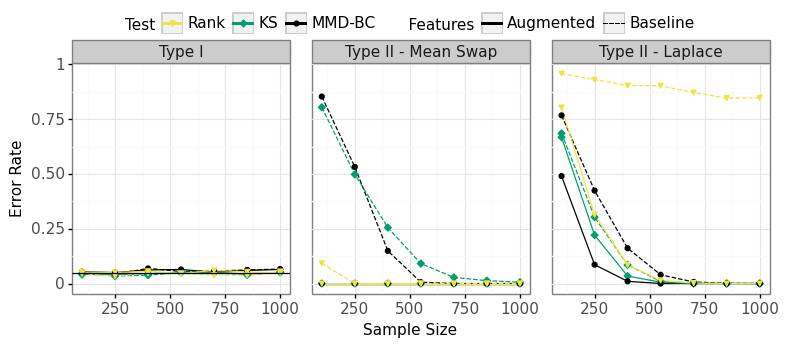
\includegraphics[width=\textwidth]{figures/results_1.png}
    \caption{
        Experiment 1 type-I/II error rates of BC tests with varying test functions over 1000 trials. 
        The red flat line in the left panel indicates the significance level $\alpha=0.05$. 
        For the BC simulator, we set the burn-in size $L=500$.
        The Rank test computes a rank statistic based on $\tilde{L}=5$ samples.
    }
    \label{fig:ex1_aux}
\end{figure}

We observed that when $\sigma_{\epsilon} \ll \sigma$, the sample autocorrelation in the successive conditional sampler is very high, and successive-conditional tests require many more samples than backwards-conditional tests to push their type-I error rates below $\alpha=0.05$. Tuning $\sigma_{\epsilon}$ thus enables analysis of test behavior given samplers with varying mixing speeds (see Appendix \ref{appendix:ex1a}). When the sample autocorrelation is very high, the MMD-SC and Geweke tests almost always reject the null hypothesis; their elevated type-I error rates can be fixed by drawing more samples or by tweaking the window size and wild bootstrap parameters, respectively. As $\sigma_{\epsilon}$ increases and the autocorrelation falls, the required adjustments become smaller; however, it is challenging to set these parameters correctly beforehand. Type-II error rates improve across all tests with mixing speed.

\subsection{Reversible-jump Bayesian Lasso}
\label{section:ex2}
We next consider a Bayesian Lasso model similar to \cite{chen_bayesian_2011}. 
Here, for a fixed design matrix $\mathbf{X}\in \mathbb{R}^{m\times d}$ with $m, d \geq 1,$ we model its associated outcome variable $Y$ with  
a linear regression model
\begin{equation}
    Y = \mathbf{X}{\beta} + \mathbf{\epsilon}, \quad \mathbf{\epsilon} \sim \mathcal{N}(\mathbf{0}, \sigma^{2} \mathbf{I}), 
    \label{eq:ex2}
\end{equation}
where ${\beta} = [\beta_1, \dots, \beta_d]^{\top} \in \mathbb{R}^d$ are sparse coefficients, $\sigma>0,$ and $\mathbf{I}$ is the identity matrix. 
To define a Bayesian model, we place a truncated Poisson prior on the number $\ell$ of nonzero elements in $\beta$ and an inverse-gamma prior on $\sigma^{2}$ with hyperparameters $a, b$. 
The model draws a combination $\gamma$ of $\ell$ integers from $\{1,\dots, d\}$, uniformly from all the combinations, to choose nonzero coefficients $\{\beta_{j}\}_{j\in \gamma}$.
The selected weights $\{\beta_{j}\}_{j\in \gamma}$ are then independently drawn from a Laplace distribution with scale $\tau$. 

% The prior is thus
% \begin{equation}
%   \pi(\theta=(\beta, \sigma)|\tau, a, b ) = p(\ell|\lambda) p(\mathbf{\gamma}|\ell) p(\sigma^{2} | a, b) \prod_{j=1}^d p(\beta_{j} | \tau, \gamma). 
% \end{equation}
For observed outcomes $y$, the model is used to infer the parameters $\theta = (\beta, \sigma)$.
Because the number of nonzero coefficients in \eqref{eq:ex2} is unknown, the algorithm must draw from parameter spaces of varying dimension. 
We implement a reversible-jump step \citep{green_reversible_1995} based on \cite{chen_bayesian_2011}; see Appendix \ref{appendix:ex2} for full details. 
The reversible jump random walk sizes are set to $\epsilon_\text{update}= \epsilon_\text{birth}=1$. Each iteration of the reversible-jump MCMC posterior sampler takes two steps in random order. A Gibbs step updates $\sigma^{2}$, which is straightforward due to the conjugacy of the inverse gamma prior on $\sigma^{2}$. A reversible-jump step traverses parameter spaces with varying $\ell$. 
We accept the birth-death proposal $\tilde{\theta}$ with probability 
\begin{equation}
    A(\tilde{\theta}|\theta) = \min{\left(\frac{p(y, \tilde{\theta} | X, \tau, a, b )}{p(y, \theta | X, \tau, a, b )} \frac{p(\tilde{\theta} \rightarrow \theta)}{p(\theta \rightarrow \tilde{\theta})}, 1\right)}.
\end{equation}

We introduce two errors into the the posterior sampler: One affects the Metropolis-Hastings acceptance probabilities used in the birth/death moves; it omits the jump probabilities $p(\tilde{\theta} \rightarrow \theta), p(\theta \rightarrow \tilde{\theta})$ from the calculation. The second error affects all of the Metropolis-Hastings acceptance probabilities. The truncated Poisson factors $p(\ell|\lambda)$  of the joint probabilities have incorrect denominator $(\ell-1)!$ rather than $\ell!$. In summary:
\begin{center}
   \begin{tabular}{llll}
                  Error & Components & Incorrect & Correct \\
    \midrule  
         Transition & $A_{\text{birth}}(\tilde{\theta}|\theta)$, $A_{\text{death}}(\tilde{\theta}|\theta)$  &  $\ldots\frac{p(y, \tilde{\theta} | X )}{p(y, \theta | X )}\ldots$ & $\ldots\frac{p(y, \tilde{\theta} | X )}{p(y, \theta | X )} \frac{p(\tilde{\theta} \rightarrow \theta)}{p(\theta \rightarrow \tilde{\theta})}\ldots$\\
         Poisson & $p(y, \tilde{\theta} | X )$, $p(y, \theta | X )$ & $\ldots \frac{\exp{(-\lambda)} \lambda^{\ell}}{(\ell-1)!} \ldots$ & $\ldots \frac{\exp{(-\lambda)} \lambda^{\ell}}{\ell!} \ldots$ \\
\end{tabular}
\end{center}    


For the MMD tests, we use the same kernel as in the previous experiment: $k_{\mathrm{IMQ}}(g, \tilde{g}) + k_{\mathrm{IMQ}}(h, \tilde{h})$. The benchmark tests use all first and second moments of $\{\beta,\sigma\}$ and the evaluations of the likelihood and prior.
We fix $m=d=3$ with $\lambda=1$, and use hyperparameters $\tau=1$, $a=3,$ and $b=1$. 
The results are shown in Figure \ref{fig:ex2_comparison}. The autocorrelation in the successive-conditional samples results in elevated rejection rates for the Geweke test. Despite using the same samples, the MMD-SC test better controls type-I error rates. Its type-II error rates are decidedly worse than the other tests, however. Due to the independence of their samples, the backwards-conditional tests are generally more efficient. The MMD-BC trails the KS test, implying that the test functions align with the errors.

% \begin{table}[b]
%     \caption{Experiment 2; summary of intentional errors in posterior sampler}
%     \label{tab:ex2_errors}
%     \centering
%     \begin{tabular}{llll}
%     \toprule
%           Error & Components & Incorrect & Correct \\
%     \midrule  
%          Transition & $A_{\text{birth}}(\tilde{\theta}|\theta)$, $A_{\text{death}}(\tilde{\theta}|\theta)$  &  $\ldots\frac{p(y, \tilde{\theta} | X )}{p(y, \theta | X )}\ldots$ & $\ldots\frac{p(y, \tilde{\theta} | X )}{p(y, \theta | X )} \frac{p(\tilde{\theta} \rightarrow \theta)}{p(\theta \rightarrow \tilde{\theta})}\ldots$\\
%          Poisson & $p(y, \tilde{\theta} | X )$, $p(y, \theta | X )$ & $\ldots \frac{\exp{(-\lambda)} \lambda^{\ell}}{(\ell-1)!} \ldots$ & $\ldots \frac{\exp{(-\lambda)} \lambda^{\ell}}{\ell!} \ldots$ \\
%     \bottomrule
%     \end{tabular}
% \end{table}

\begin{figure}
    \centering
    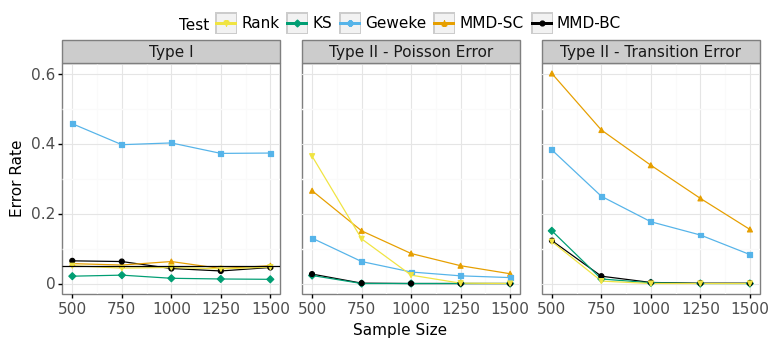
\includegraphics[width=\textwidth]{figures/results_2.png}
    \caption{Experiment 2 type-I/II error rates over 1000 trials. 
    The red flat line in the left panel indicates the significance level $\alpha=0.05$. 
    We set the thinning size $t=5$ for the SC simulator, and $L=500$ for both the SC and BC simulators. For the Rank test, we set the burn-in size $\tilde{L}=5$. We set the Geweke window size to $8\%$ of the sample size.
    }
    \label{fig:ex2_comparison}
\end{figure}

\subsection{Metropolis-Hastings for Learning DAG Structure} \label{sec:graphexp}
We consider a graph structure to demonstrate that the MMD tests can be easily generalized to non-Euclidean domains with a suitable kernel.
% We consider a simple model to infer the structure $\mathcal{G}$ of a directed acyclic graph (DAG) underlying observed data; 
Suppose that data $Y=(Y^1, \dots, Y^d)$ takes values in $\mathbb{R}^d.$ 
We use a model specified by a directed acyclic graph (DAG) $\mathcal{G}$, where 
$\mathcal{G}$ is a set of $d$ nodes and directed edges; 
each node represents a component of $Y$ and edges encode conditional independence relationships between node variables. 
% A root node has no parents. Note that in acyclic graphs, a node cannot be descended from itself. 
The generative process is defined as follows. 
We represent a DAG $\mathcal{G}$ by a $d\times d$ adjacency matrix; entry $(i,j)=1$ indicates that node $i$ is the parent of child node $j$, and $(i,j)=0$ otherwise. 
We set a uniform prior $\pi(\mathcal{G}) \propto 1,$ which may be sampled from using the algorithm in \cite{kuipers_uniform_2015}. 
% Let $\mathbf{pa}(y)$ denote the set of parent nodes of node $y$. 
Given a DAG $\mathcal{G}$, we draw each root node variable from $\mathcal{N}(0, \epsilon^2)$, and each child node $Y^{c}$ from $\mathcal{N}(\sum_{z \in \mathbf{p}_c} z, \epsilon^2)$ with $\mathbf{p}_c$ the set of parent nodes of the child node $c.$ 
% The likelihood is thus $    p(y|\mathcal{G}) = \prod_{j=1}^{n}  p(y_{j}|\mathcal{G}) = \prod_{j=1}^{n} p(y_{j}|\mathbf{pa}(y_{j}))$.

To infer $\mathcal{G}$ given observed data, we use the MCMC algorithm detailed in Section 2 of \cite{grzegorczyk_improving_2008}; 
Given a structure $\mathcal{G}$, the proposal structure $\mathcal{G}'$ is sampled uniformly from the neighborhood $\mathbf{Ne}(\mathcal{G})$, the union of $\mathcal{G}$ and the set of all DAGs that can be reached by adding, deleting, or reversing an edge. 
We consider a sampler error affecting the Metropolis-Hastings acceptance probability
\begin{equation}
A(\tilde{\mathcal{G}}|\mathcal{G}) = \min{\left(\frac{p(y|\tilde{\mathcal{G}})|\mathbf{Ne}(\mathcal{G})|}{p(y|\mathcal{G})|\mathbf{Ne}(\tilde{\mathcal{G}})|}, 1\right)}. \label{eq:exp_graph_mh}
\end{equation}
Specifically, it alters the calculation of the number of the neighborhood nodes $|\mathbf{Ne}(\mathcal{G})|$: we count all \textit{graphs} that can be reached by modifying a single edge, regardless of whether the modification induces a cycle. 
\begin{center}
    \begin{tabular}{llll}
    Error & Components & Incorrect & Correct \\
    \midrule  
         Cyclic Check & $|\mathbf{Ne}(\mathcal{G})|, |\mathbf{Ne}(\mathcal{G}')|$ & Count graph neighbors & Count DAG neighbors \\
        %  Rev Count & $|\mathbf{Ne}(\mathcal{G})|, |\mathbf{Ne}(\mathcal{G}')|$ & Count reversals twice & Count reversals once \\
    \end{tabular}
\end{center}
% In the first error, we count all \textit{graphs} that can be reached by modifying a single edge, regardless of whether the modification induces a cycle. In the subtler second error, we double-count the DAGs that can be reached by reversing an edge. 

% \begin{table}[t]
%     \caption{Experiment 3; summary of intentional errors in posterior sampler}
%     \label{tab:ex3_errors}
%     \centering
%     \begin{tabular}{llll}
%     \toprule
%           Error & Components & Incorrect & Correct \\
%     \midrule  
%          Cyclic Check & $|\mathbf{Ne}(\mathcal{G})|, |\mathbf{Ne}(\mathcal{G}')|$ & Count graph neighbors & Count DAG neighbors \\
%         %  Rev Count & $|\mathbf{Ne}(\mathcal{G})|, |\mathbf{Ne}(\mathcal{G}')|$ & Count reversals twice & Count reversals once \\
%     \bottomrule
%     \end{tabular}
% \end{table}

We examine two sets of tests: one with Euclidean features and the other with graph features. 
For the former, we treat each entry in the adjacency matrix of the sampled graph $\mathcal{G}$ as a binary parameter and use the likelihood $p(y|\mathcal{G})$ as our auxiliary test function. 
For the Geweke test, we use a subset of the the first and second moments of these parameters as test functions; we exclude duplicate moments and all moments that must be zero for the graph to be acyclic. 
The KS test uses the same test functions with a permutation bootstrap to simulate the null parameter distributions.
For the MMD tests, we use the IMQ sum kernel from previous experiments and center the adjacency matrix entries around zero to avoid disappearing terms in the IMQ kernel evaluations. 
%%%%%%%%%%%%%%%%%%
% the following details should be used for interpreting the results, but not for providing experiment specifics 
% Under the adjacency matrix representation, the number of first and second moments is quadratic in the number of nodes; the Geweke test will eventually lose power from multiple testing corrections, as the number of node variables increases. 
% For the MMD tests, the number of test functions scales quadratically; the high dimension will shrink the test statistic and reduce power.
%%%%%%%%%%%%%%%%%%

For the latter, we consider the MMD tests with the random walk (RW) kernel \citep{gartner_graph_2003, vishwanathan_fast_2006} implemented in \cite{siglidis_grakel_2020}. 
We also considered a sum of normalized kernels $(\tilde{k}(x, x') = k(x, x')/\sqrt{k(x,x) k(x',x')})$ to combine the RW, joint IMQ, and auxiliary IMQ kernels; the results were similar to the the foregoing IMQ-kernel MMD tests and are therefore omitted. Another benchmark is the rank test, using a random tiebreak to sort the generated graphs directly as well as the likelihood. 
As an idealized benchmark in the graph space, we include a $\chi^{2}$ test of backwards-conditional sample DAG frequencies; this uses the true prior frequencies, which should be recovered by the aggregated posterior.
\begin{figure}[t]
    \centering
    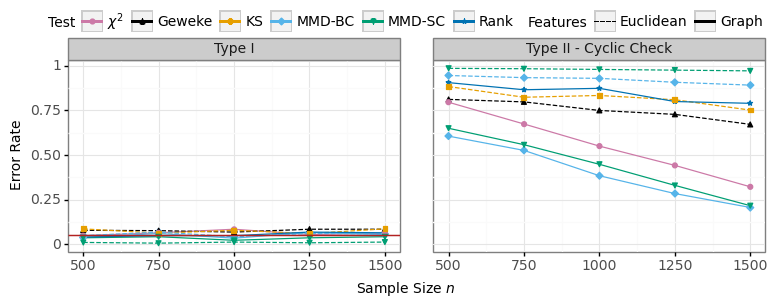
\includegraphics[width=\textwidth]{figures/results_3.png}
    \caption{Experiment 3 type-I/II error rates over 500 trials. 
    The red flat line in the left panel indicates the significance level $\alpha=0.05$. 
    The thinning size $t$ is set to $5$ for the SC simulator, and the burn-in size $L=500$ is used for both the SC and BC simulators. The Geweke window size was set to $8\%$ of the sample size. 
    }
    % For the Geweke test, we use a subset of the the first and second moments of these parameters as test functions; all moments that must be zero for the graph to be cyclic are excluded.
    \label{fig:ex3_comparison}
\end{figure}
Figure \ref{fig:ex3_comparison} shows the results. 
The Geweke test outperforms the MMD tests with the IMQ kernel; in contrast, using the RW kernel, the MMD tests outperform the Geweke test and even the $\chi^{2}$ test in detecting the Cyclic Check error. 

\section{Conclusion}
\label{sec:conclusion}
We have developed a nonparametric extension of Geweke's test using the MMD.   
The advantage of the new test is its simplicity; with a suitable kernel, the test does not require manual specification of test functions and is not limited to Euclidean space, while care needs to be taken otherwise. The trade-off, however, is that characteristic kernels are challenging to compute in certain domains.
For example, in graphs the delta kernel examining if two graphs are identical is computationally intractable for large graphs. 
RW kernels, and other fast alternatives, cannot distinguish between isomorphic graphs. 
With an RW kernel, when the null hypothesis is not rejected even with a large sample, it should be understood that the joint distributions could still have differences indiscernible to the test. 
In fact, we found that the MMD test with the RW kernel in Section \ref{sec:graphexp} had low power when slightly increasing only the reversal counts in the neighborhood in \eqref{eq:exp_graph_mh}. 
Such limitations, however, may not matter if the posterior is invariant under graph isomorphisms. 
In sum, when choosing a kernel, the user should take into account what features the test can distinguish with it, and whether those features are relevant to the problem; the test result should be interpreted accordingly. 
Finally, the test inherits limitations and caveats of frequentist hypothesis testing; e.g., the $p$-value is not the probability of the null hypothesis being true, and non-rejection of the null does not imply that the null is true. 
% The advantage of the MMD tests here is its simplicity; we can apply the same tests in $\mathbb{R}^{d}$, graph space, or a mix of the two; all we need to do is change the kernel. 
% In fact, random walk kernels cannot distinguish between isomorphic graphs.
% The primary concern outside of $\mathbb{R}^{d}$ is that, if we do not have access to characteristic kernels, the consistency of the MMD tests is not guaranteed.
% Note that this lack of consistency is shared by the benchmark tests. While the $\chi^{2}$ test performs best in the Rev Count type-II error, offering a consistent test of the aggregate posterior for a linear computational cost, prior recovery is not sufficient for sampler correctness, as discussed in Section \ref{related:work}. 
% In addition, it may only be applied when the parameter space is discrete. Similarly, the Geweke test is limited by its test functions. 
% Taking the sum kernel composed of the random walk, joint IMQ, and auxiliary IMQ kernels, with normalized components of the form $\tilde{k}(x, x') = k(x, x')/\sqrt{k(x,x) k(x',x')}$, gave similar results to the IMQ sum kernel.

\section{Broader Impact}
\label{sec:impact}
MCMC algorithms are commonly used across the natural and social sciences. However, they can be quite complex and error-prone. Compared to other methods, our diagnostics come with improved theoretical guarantees as well as wider and more convenient applicability; they are thus are of practical use to both researchers and practitioners. They may reduce error propagation in related academic literature by easing detection of existing mistakes and preventing the introduction of new ones.

% \subsection{Style}

% Papers to be submitted to NeurIPS 2021 must be prepared according to the
% instructions presented here. Papers may only be up to {\bf nine} pages long,
% including figures. Additional pages \emph{containing only acknowledgments and
% references} are allowed. Papers that exceed the page limit will not be
% reviewed, or in any other way considered for presentation at the conference.

% The margins in 2021 are the same as those in 2007, which allow for $\sim$$15\%$
% more words in the paper compared to earlier years.

% Authors are required to use the NeurIPS \LaTeX{} style files obtainable at the
% NeurIPS website as indicated below. Please make sure you use the current files
% and not previous versions. Tweaking the style files may be grounds for
% rejection.

% \subsection{Retrieval of style files}

% The style files for NeurIPS and other conference information are available on
% the World Wide Web at
% \begin{center}
%   \url{http://www.neurips.cc/}
% \end{center}
% The file \verb+neurips_2021.pdf+ contains these instructions and illustrates the
% various formatting requirements your NeurIPS paper must satisfy.

% The only supported style file for NeurIPS 2021 is \verb+neurips_2021.sty+,
% rewritten for \LaTeXe{}.  \textbf{Previous style files for \LaTeX{} 2.09,
%   Microsoft Word, and RTF are no longer supported!}

% The \LaTeX{} style file contains three optional arguments: \verb+final+, which
% creates a camera-ready copy, \verb+preprint+, which creates a preprint for
% submission to, e.g., arXiv, and \verb+nonatbib+, which will not load the
% \verb+natbib+ package for you in case of package clash.

% \paragraph{Preprint option}
% If you wish to post a preprint of your work online, e.g., on arXiv, using the
% NeurIPS style, please use the \verb+preprint+ option. This will create a
% nonanonymized version of your work with the text ``Preprint. Work in progress.''
% in the footer. This version may be distributed as you see fit. Please \textbf{do
%   not} use the \verb+final+ option, which should \textbf{only} be used for
% papers accepted to NeurIPS.

% At submission time, please omit the \verb+final+ and \verb+preprint+
% options. This will anonymize your submission and add line numbers to aid
% review. Please do \emph{not} refer to these line numbers in your paper as they
% will be removed during generation of camera-ready copies.

% The file \verb+neurips_2021.tex+ may be used as a ``shell'' for writing your
% paper. All you have to do is replace the author, title, abstract, and text of
% the paper with your own.

% The formatting instructions contained in these style files are summarized in
% Sections \ref{gen_inst}, \ref{headings}, and \ref{others} below.

% \section{General formatting instructions}
% \label{gen_inst}

% The text must be confined within a rectangle 5.5~inches (33~picas) wide and
% 9~inches (54~picas) long. The left margin is 1.5~inch (9~picas).  Use 10~point
% type with a vertical spacing (leading) of 11~points.  Times New Roman is the
% preferred typeface throughout, and will be selected for you by default.
% Paragraphs are separated by \nicefrac{1}{2}~line space (5.5 points), with no
% indentation.

% The paper title should be 17~point, initial caps/lower case, bold, centered
% between two horizontal rules. The top rule should be 4~points thick and the
% bottom rule should be 1~point thick. Allow \nicefrac{1}{4}~inch space above and
% below the title to rules. All pages should start at 1~inch (6~picas) from the
% top of the page.

% For the final version, authors' names are set in boldface, and each name is
% centered above the corresponding address. The lead author's name is to be listed
% first (left-most), and the co-authors' names (if different address) are set to
% follow. If there is only one co-author, list both author and co-author side by
% side.

% Please pay special attention to the instructions in Section \ref{others}
% regarding figures, tables, acknowledgments, and references.

% \section{Headings: first level}
% \label{headings}

% All headings should be lower case (except for first word and proper nouns),
% flush left, and bold.

% First-level headings should be in 12-point type.

% \subsection{Headings: second level}

% Second-level headings should be in 10-point type.

% \subsubsection{Headings: third level}

% Third-level headings should be in 10-point type.

% \paragraph{Paragraphs}

% There is also a \verb+\paragraph+ command available, which sets the heading in
% bold, flush left, and inline with the text, with the heading followed by 1\,em
% of space.

% \section{Citations, figures, tables, references}
% \label{others}

% These instructions apply to everyone.

% \subsection{Citations within the text}

% The \verb+natbib+ package will be loaded for you by default.  Citations may be
% author/year or numeric, as long as you maintain internal consistency.  As to the
% format of the references themselves, any style is acceptable as long as it is
% used consistently.

% The documentation for \verb+natbib+ may be found at
% \begin{center}
%   \url{http://mirrors.ctan.org/macros/latex/contrib/natbib/natnotes.pdf}
% \end{center}
% Of note is the command \verb+\citet+, which produces citations appropriate for
% use in inline text.  For example,
% \begin{verbatim}
%   \citet{hasselmo} investigated\dots
% \end{verbatim}
% produces
% \begin{quote}
%   Hasselmo, et al.\ (1995) investigated\dots
% \end{quote}

% If you wish to load the \verb+natbib+ package with options, you may add the
% following before loading the \verb+neurips_2021+ package:
% \begin{verbatim}
% \PassOptionsToPackage{options}{natbib}
% \end{verbatim}

% If \verb+natbib+ clashes with another package you load, you can add the optional
% argument \verb+nonatbib+ when loading the style file:
% \begin{verbatim}
%   \usepackage[nonatbib]{neurips_2021}
% \end{verbatim}

% As submission is double blind, refer to your own published work in the third
% person. That is, use ``In the previous work of Jones et al.\ [4],'' not ``In our
% previous work [4].'' If you cite your other papers that are not widely available
% (e.g., a journal paper under review), use anonymous author names in the
% citation, e.g., an author of the form ``A.\ Anonymous.''

% \subsection{Footnotes}

% Footnotes should be used sparingly.  If you do require a footnote, indicate
% footnotes with a number\footnote{Sample of the first footnote.} in the
% text. Place the footnotes at the bottom of the page on which they appear.
% Precede the footnote with a horizontal rule of 2~inches (12~picas).

% Note that footnotes are properly typeset \emph{after} punctuation
% marks.\footnote{As in this example.}

% \subsection{Figures}

% \begin{figure}
%   \centering
%   \fbox{\rule[-.5cm]{0cm}{4cm} \rule[-.5cm]{4cm}{0cm}}
%   \caption{Sample figure caption.}
% \end{figure}

% All artwork must be neat, clean, and legible. Lines should be dark enough for
% purposes of reproduction. The figure number and caption always appear after the
% figure. Place one line space before the figure caption and one line space after
% the figure. The figure caption should be lower case (except for first word and
% proper nouns); figures are numbered consecutively.

% You may use color figures.  However, it is best for the figure captions and the
% paper body to be legible if the paper is printed in either black/white or in
% color.

% \subsection{Tables}

% All tables must be centered, neat, clean and legible.  The table number and
% title always appear before the table.  See Table~\ref{sample-table}.

% Place one line space before the table title, one line space after the
% table title, and one line space after the table. The table title must
% be lower case (except for first word and proper nouns); tables are
% numbered consecutively.

% Note that publication-quality tables \emph{do not contain vertical rules.} We
% strongly suggest the use of the \verb+booktabs+ package, which allows for
% typesetting high-quality, professional tables:
% \begin{center}
%   \url{https://www.ctan.org/pkg/booktabs}
% \end{center}
% This package was used to typeset Table~\ref{sample-table}.

% \begin{table}
%   \caption{Sample table title}
%   \label{sample-table}
%   \centering
%   \begin{tabular}{lll}
%     \toprule
%     \multicolumn{2}{c}{Part}                   \\
%     \cmidrule(r){1-2}
%     Name     & Description     & Size ($\mu$m) \\
%     \midrule
%     Dendrite & Input terminal  & $\sim$100     \\
%     Axon     & Output terminal & $\sim$10      \\
%     Soma     & Cell body       & up to $10^6$  \\
%     \bottomrule
%   \end{tabular}
% \end{table}

% \section{Final instructions}

% Do not change any aspects of the formatting parameters in the style files.  In
% particular, do not modify the width or length of the rectangle the text should
% fit into, and do not change font sizes (except perhaps in the
% \textbf{References} section; see below). Please note that pages should be
% numbered.

% \section{Preparing PDF files}

% Please prepare submission files with paper size ``US Letter,'' and not, for
% example, ``A4.''

% Fonts were the main cause of problems in the past years. Your PDF file must only
% contain Type 1 or Embedded TrueType fonts. Here are a few instructions to
% achieve this.

% \begin{itemize}

% \item You should directly generate PDF files using \verb+pdflatex+.

% \item You can check which fonts a PDF files uses.  In Acrobat Reader, select the
%   menu Files$>$Document Properties$>$Fonts and select Show All Fonts. You can
%   also use the program \verb+pdffonts+ which comes with \verb+xpdf+ and is
%   available out-of-the-box on most Linux machines.

% \item The IEEE has recommendations for generating PDF files whose fonts are also
%   acceptable for NeurIPS. Please see
%   \url{http://www.emfield.org/icuwb2010/downloads/IEEE-PDF-SpecV32.pdf}

% \item \verb+xfig+ "patterned" shapes are implemented with bitmap fonts.  Use
%   "solid" shapes instead.

% \item The \verb+\bbold+ package almost always uses bitmap fonts.  You should use
%   the equivalent AMS Fonts:
% \begin{verbatim}
%   \usepackage{amsfonts}
% \end{verbatim}
% followed by, e.g., \verb+\mathbb{R}+, \verb+\mathbb{N}+, or \verb+\mathbb{C}+
% for $\mathbb{R}$, $\mathbb{N}$ or $\mathbb{C}$.  You can also use the following
% workaround for reals, natural and complex:
% \begin{verbatim}
%   \newcommand{\RR}{I\!\!R} %real numbers
%   \newcommand{\Nat}{I\!\!N} %natural numbers
%   \newcommand{\CC}{I\!\!\!\!C} %complex numbers
% \end{verbatim}
% Note that \verb+amsfonts+ is automatically loaded by the \verb+amssymb+ package.

% \end{itemize}

% If your file contains type 3 fonts or non embedded TrueType fonts, we will ask
% you to fix it.

% \subsection{Margins in \LaTeX{}}

% Most of the margin problems come from figures positioned by hand using
% \verb+\special+ or other commands. We suggest using the command
% \verb+\includegraphics+ from the \verb+graphicx+ package. Always specify the
% figure width as a multiple of the line width as in the example below:
% \begin{verbatim}
%   \usepackage[pdftex]{graphicx} ...
%   \includegraphics[width=0.8\linewidth]{myfile.pdf}
% \end{verbatim}
% See Section 4.4 in the graphics bundle documentation
% (\url{http://mirrors.ctan.org/macros/latex/required/graphics/grfguide.pdf})

% A number of width problems arise when \LaTeX{} cannot properly hyphenate a
% line. Please give LaTeX hyphenation hints using the \verb+\-+ command when
% necessary.

\begin{ack}
Use unnumbered first level headings for the acknowledgments. All acknowledgments
go at the end of the paper before the list of references. Moreover, you are required to declare
funding (financial activities supporting the submitted work) and competing interests (related financial activities outside the submitted work).
More information about this disclosure can be found at: \url{https://neurips.cc/Conferences/2021/PaperInformation/FundingDisclosure}.

Do {\bf not} include this section in the anonymized submission, only in the final paper. You can use the \texttt{ack} environment provided in the style file to autmoatically hide this section in the anonymized submission.
\end{ack}

% \section*{References}
\small{
\bibliography{references}
% [1] Alexander, J.A.\ \& Mozer, M.C.\ (1995) Template-based algorithms for
% connectionist rule extraction. In G.\ Tesauro, D.S.\ Touretzky and T.K.\ Leen
% (eds.), {\it Advances in Neural Information Processing Systems 7},
% pp.\ 609--616. Cambridge, MA: MIT Press.

% [2] Bower, J.M.\ \& Beeman, D.\ (1995) {\it The Book of GENESIS: Exploring
%   Realistic Neural Models with the GEneral NEural SImulation System.}  New York:
% TELOS/Springer--Verlag.

% [3] Hasselmo, M.E., Schnell, E.\ \& Barkai, E.\ (1995) Dynamics of learning and
% recall at excitatory recurrent synapses and cholinergic modulation in rat
% hippocampal region CA3. {\it Journal of Neuroscience} {\bf 15}(7):5249-5262.
}

%%%%%%%%%%%%%%%%%%%%%%%%%%%%%%%%%%%%%%%%%%%%%%%%%%%%%%%%%%%%
\section*{Checklist}

% %%% BEGIN INSTRUCTIONS %%%
% The checklist follows the references.  Please
% read the checklist guidelines carefully for information on how to answer these
% questions.  For each question, change the default \answerTODO{} to \answerYes{},
% \answerNo{}, or \answerNA{}.  You are strongly encouraged to include a {\bf
% justification to your answer}, either by referencing the appropriate section of
% your paper or providing a brief inline description.  For example:
% \begin{itemize}
%   \item Did you include the license to the code and datasets? \answerYes{See Section~\ref{gen_inst}.}
%   \item Did you include the license to the code and datasets? \answerNo{The code and the data are proprietary.}
%   \item Did you include the license to the code and datasets? \answerNA{}
% \end{itemize}
% Please do not modify the questions and only use the provided macros for your
% answers.  Note that the Checklist section does not count towards the page
% limit.  In your paper, please delete this instructions block and only keep the
% Checklist section heading above along with the questions/answers below.
% %%% END INSTRUCTIONS %%%

\begin{enumerate}

\item For all authors...
\begin{enumerate}
  \item Do the main claims made in the abstract and introduction accurately reflect the paper's contributions and scope?
    \answerYes{}
  \item Did you describe the limitations of your work?
    \answerYes{}
  \item Did you discuss any potential negative societal impacts of your work?
    \answerNA{}
  \item Have you read the ethics review guidelines and ensured that your paper conforms to them?
    \answerYes{See Section \ref{sec:conclusion}}
\end{enumerate}

\item If you ran experiments...
\begin{enumerate}
  \item Did you include the code, data, and instructions needed to reproduce the main experimental results (either in the supplemental material or as a URL)?
    \answerYes{Will be included in supplemental material}
  \item Did you specify all the training details (e.g., data splits, hyperparameters, how they were chosen)?
    \answerYes{Any additional details will be included in supplemental materials}
	\item Did you report error bars (e.g., with respect to the random seed after running experiments multiple times)?
    \answerNA{}{}
	\item Did you include the total amount of compute and the type of resources used (e.g., type of GPUs, internal cluster, or cloud provider)?
    \answerNA{}
\end{enumerate}

\item If you are using existing assets (e.g., code, data, models) or curating/releasing new assets...
\begin{enumerate}
  \item If your work uses existing assets, did you cite the creators?
    \answerYes{Cited \cite{siglidis_grakel_2020}}
  \item Did you mention the license of the assets?
    \answerYes{Will be included in supplemental materials}
  \item Did you include any new assets either in the supplemental material or as a URL?
    \answerYes{Will be included in supplemental materials}
  \item Did you discuss whether and how consent was obtained from people whose data you're using/curating?
    \answerNA{}
  \item Did you discuss whether the data you are using/curating contains personally identifiable information or offensive content?
    \answerNA{}
\end{enumerate}

\end{enumerate}
\newpage
\appendix

\section{Baseline methods}
\subsection{Geweke test}
The Geweke test \citep{geweke_getting_2004} compares (estimates of) the expectations of hand-picked features (\emph{test functions}) under both the forward and backward joints. 
Specifically, let $g: \mathcal{Y}\times \Theta\to \mathbb{R}$ denote a test function, and let  $S_f=\{(y_i, \theta_i)\}_{i=1}^n$ be samples from the forward joint and $S_b=\{(\tilde{y}_i, \tilde{\theta}_i)\}_{i=1}^n$ be ones from the backward joint.
Then, the z-score 
% $\sqrt{n}(\hat{\bar{g}} - \hat{\tilde{g}})/\sqrt{\hat{\sigma^{2}}+\hat{\tilde{\sigma}}^{2}}$
\begin{equation}
    \frac{\bar{g}(S_f) - \bar{g}(S_b)}{\sqrt{ \frac{\hat{\sigma}^{2}}{N} + \frac{\hat{\tilde{\sigma}}^{2}}{N}}} 
    % \xrightarrow[]{d} \mathcal{N}(0, 1)
    \label{eq:geweke}
\end{equation}
asymptotically follows the standard Gaussian if $\tilde{\pi}(\theta\given y)=\pi(\theta\given y)$, where $\bar{g}(S) = \frac{1}{n}\sum_{(y,\theta) \in S}g(y, \theta)$ and $\hat{\sigma}, \hat{\tilde{\sigma}}$ are estimated variances. 
The width of the window estimator $\hat{\tilde{\sigma}}$ can be set to account for the serial dependence in the backward joint samples.
\subsection{\cite{talts_validating_2018}}
% \cite{talts_validating_2018} take a similar approach under the assumption that the posterior is absolutely continuous.
The authors draw samples using the BC algorithm, then compute univariate rank statistics of a draw from the prior among the thinned, approximately independent posterior samples; if there is no error, the rank statistics should be discretely uniformly distributed. 
The authors suggest examining histograms of the rank statistics to better understand errors rather than conducting a formal test.

\subsection{Rank statistic approach of \cite{gandy_unit_2020}}
The rank test from \cite{gandy_unit_2020} requires reversibility of the MCMC sampler. It draws a sample $\theta_{l}$ from the prior, with the associated index $l$ drawn uniformly from $\{1,\ldots,\tilde{L}\}$. The sampler is then run forward and backward to generate samples $\theta_{1}, \ldots, \theta_{l-1}$ and $\theta_{l+1}, \ldots, \theta_{\tilde{L}} $. Under the null, the rank statistic of $\theta_{l}$ among the other samples should be uniformly distributed; after many repeated simulations, this is verified using a $\chi^{2}$ test.

\section{Experiment details}
\subsection{Experiment 1}
\subsubsection{Effect of sampler mixing speed}
\label{appendix:ex1a}
\begin{figure}[H]
    \centering
    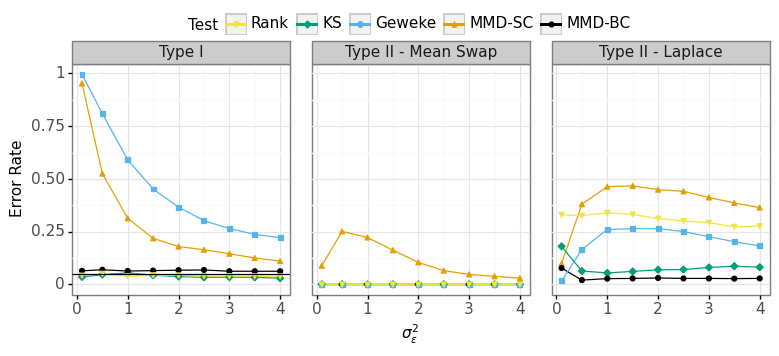
\includegraphics[width=\textwidth]{figures/results_1a.png}
    \caption{Experiment 1 type-I/II error rates against $\sigma_{\epsilon}$, over 1000 trials with a sample size of 250. As $\sigma_{\epsilon}$ increases, autocorrelation in the Gibbs sampler decreases and mixing speed increases. We use the thinning size $t=5$ for the SC simulator, and take $L=500$ burn-in steps for both the SC and BC simulators. For the Rank test, each rank statistic is calculated using a chain of length $\tilde{L}=5$.}
    \label{fig:ex1a}
\end{figure}

\subsubsection{Effect of varying BC simulator burn-in}
\begin{figure}[H]
    \centering
    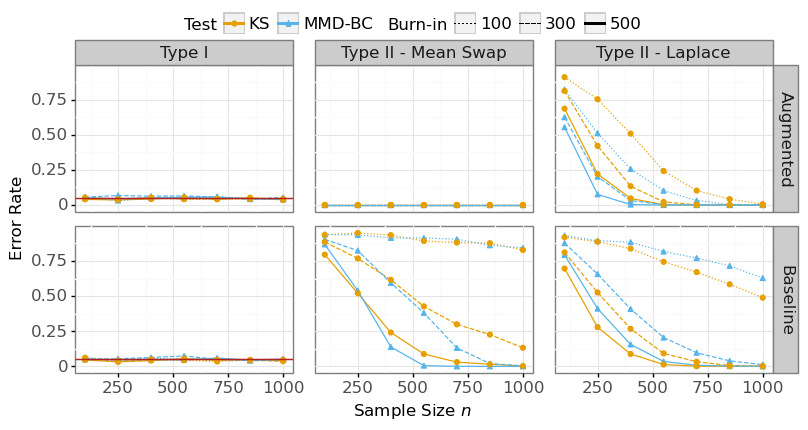
\includegraphics[width=\textwidth]{figures/results_1b.png}
    \caption{Experiment 1 type-I/II error rates over 1000 trials for different burn-in sizes $L$. The top panels use the likelihood- and prior-augmented test functions and the bottom panels use the baseline as discussed in the text. We set $\sigma_{\epsilon}^{2}=0.1$. Type-II error rates fall as the $L$ increases.}
    \label{fig:ex2b}
\end{figure}

\subsection{Experiment 2: Reversible Jump Sampler Implementation}
\label{appendix:ex2}
The prior is defined by
\begin{equation}
  \pi(\theta|\tau, a, b ) = p(\ell|\lambda) p(\mathbf{\gamma}|\ell) p(\sigma^{2} | a, b) \prod_{j} p(\beta_{j} | \tau, \gamma) 
\end{equation}
where
\begin{equation}
  p(\ell|\lambda) = \frac{\exp{(-\lambda)} \lambda^{\ell}}{C\ell!}, \quad \ell \in \{1,\ldots, p\}
\end{equation}
\begin{equation}
  p(\mathbf{\gamma}|\ell) \propto {d\choose \ell}^{-1}
\end{equation}
\begin{equation}
  p(\beta_{j} | \tau, \gamma ) = \begin{cases} (2\tau)^{-1}\exp(-\frac{|\beta_{j}|}{\tau}) & j \in \mathbf{\gamma} \\ \delta(\beta_{j}) & \text{otherwise} \end{cases}
\end{equation}
\begin{equation}
    p(\sigma^{2} | a, b) = \frac{b^{a}}{\Gamma(a)} (\sigma^{2})^{-a-1} \exp{\left(-\frac{b}{\sigma^{2}}\right)}
\end{equation}
$C$ is a normalization constant, $\delta$ is the Dirac delta function, and $\mathbf{\gamma}$ is a vector of the nonzero indices of $\beta$.
The likelihood is given by
\begin{equation}
  p(y | \sigma, \beta, X ) = (2\pi)^{-\frac{n}{2}} \sigma^{-n} \exp{\left(-\frac{\Vert y-X\beta\Vert^{2}_{2}}{2\sigma^{2}}\right)}
\end{equation}
The joint probability is then
\begin{equation}
    \begin{aligned}
         p(y, \theta | X ) \propto &\sigma^{-n} \exp{\left(-\frac{\Vert  y-X\beta\Vert^{2}_{2}}{2\sigma^{2}}\right)} \times \\ 
         & \frac{\exp{(-\lambda)} \lambda^{\ell}}{\ell!} {d\choose \ell}^{-1} \prod_{j\in \mathbf{\gamma}} (2\tau)^{-1}\exp\left(-\frac{|\beta_{j}|}{\tau}\right) \prod_{j' \notin \mathbf{\gamma}} \delta(\beta_{j'}) \frac{b^{a}}{\Gamma(a)} (\sigma^{2})^{-a-1} \exp{\left(-\frac{b}{\sigma^{2}}\right)}
    \end{aligned}
    \label{eq:ex2_joint}
\end{equation}

Each iteration of the reversible-jump MCMC posterior sampler takes two steps in random order. The first is a Gibbs step. By conjugacy,
\begin{equation}
    \sigma^{2} | y, X, \beta \sim \mathcal{IG}\left(a + \frac{n}{2}, b + \frac{\sum_{i=1}^{n}(y_{i}-x_{i}\beta)^{2} }{2}\right)
\end{equation}
where $x_{i}$ denotes row $i$ of $X$.

The second is a reversible jump step. We start by proposing $\ell' \in \{\ell-1, \ell, \ell+1\}$ uniformly at random, disallowing $\ell<1$ and $\ell>p$. Thus, when $\ell \in \{1,p\}$, there are only two valid proposals, not three. Then, depending on the $\ell'$ proposed, we complete the proposal $\tilde{\theta}$ via one of the following
\begin{itemize}
    \item Update: $\ell' = \ell$
    \begin{enumerate}
        \item Choose $j \in \{1, \ldots, \ell\}$ uniformly at random
        \item Propose $\mathbf{\gamma}' = \mathbf{\gamma}, \beta'_{j} = \beta_{j} + \mathcal{N}(0, \epsilon_{\text{update}}), \beta'_{i \neq j} = \beta_{i}$
        \item $P(\tilde{\theta} \rightarrow \theta) = P(\theta \rightarrow \tilde{\theta})=\mathcal{N}(\beta_{j}'; \beta_{j},\epsilon_{\text{update}})=\mathcal{N}(\beta_{j}; \beta_{j}',\epsilon_{\text{update}})$
    \end{enumerate}
\end{itemize}

\begin{itemize}
    \item Birth: $\ell' = \ell+1$
    \begin{enumerate}
        \item Choose $j \in \{\ell+1, \ldots, p\}$ uniformly at random
        \item Propose $\mathbf{\gamma}' = \mathbf{\gamma} \cup j$
        \item Propose $\beta'_{j} = \mathcal{N}(0, \epsilon_{\text{birth}}), \beta'_{i \neq j} = \beta_{i}$
        \item $p(\tilde{\theta} \rightarrow \theta) = \begin{cases}\frac{1}{2}\frac{1}{\ell'} & \ell'=p \\ \frac{1}{3} \frac{1}{\ell'} & 1<\ell<p \end{cases} $
        \item $p(\theta \rightarrow \tilde{\theta}) = \begin{cases}\frac{1}{2}\frac{1}{p-\ell} \mathcal{N}(\beta_{j}'; 0,\epsilon_{\text{birth}}) & \ell=1 \\ \frac{1}{3} \frac{1}{p-\ell} \mathcal{N}(\beta_{j}'; 0,\epsilon_{\text{birth}}) & 1<\ell<p \end{cases} $
    \end{enumerate}
\end{itemize}

\begin{itemize}
    \item Death: $\ell' = \ell-1$
    \begin{enumerate}
        \item Choose $j \in \{1, \ldots, \ell\}$ uniformly at random
        \item Propose $\mathbf{\gamma}' = \mathbf{\gamma} \setminus j$ 
        \item Propose $\beta'_{j} = 0, \beta'_{i \neq j} = \beta_{i}$
        \item $p(\tilde{\theta} \rightarrow \theta) = \begin{cases}\frac{1}{2}\frac{1}{p-\ell'} \mathcal{N}(\beta_{j}; 0,\epsilon_{\text{birth}}) & k'=1 \\ \frac{1}{3} \frac{1}{p-\ell'} \mathcal{N}(\beta_{j}; 0,\epsilon_{\text{birth}}) & 1<\ell'<p \end{cases} $
        \item $p(\theta \rightarrow \tilde{\theta}) = \begin{cases}\frac{1}{2}\frac{1}{\ell} & \ell=p \\ \frac{1}{3} \frac{1}{\ell} & 1<\ell<p \end{cases} $
    \end{enumerate}
\end{itemize}
where $\epsilon_{\text{update}}, \epsilon_{\text{birth}}$ are random walk sizes.

We accept the birth-death proposal $\tilde{\theta}$ with probability 
\begin{equation}
    A(\tilde{\theta}|\theta) = \min{\left(\frac{p(y, \tilde{\theta} |  X, \tau, a, b  )}{p(y, \theta |  X, \tau, a, b  )} \frac{p(\tilde{\theta} \rightarrow \theta)}{p(\theta \rightarrow \tilde{\theta})}, 1\right)} \\
\end{equation}



\end{document}
